\section{Results and Discussion}

This section presents a comprehensive analysis of our model evaluation results about the most effective approach for forecasting monthly electricity consumption in France. We examine detailed accuracy metrics and visual diagnostics for each statistical time series model — the Automatic SARIMA, Manual SARIMA, STL Decomposition followed by ARIMA (STLM), and Exponential Smoothing State Space Model (ETS) — to identify the model that delivers the most reliable and robust forecasts.

\subsection{Model Comparison Based on Information Criteria}


In addition to error metrics, information criteria such as AIC (Akaike Information Criterion), AICc (corrected AIC) and BIC (Bayesian Information Criterion) are fundamental to assessing model fit, considering adherence to the data and model complexity.

These criteria penalise overly complex models and help avoid overfitting. They are particularly useful for comparing models fitted to the same set of data.

\begin{figure}[H]
    \centering
    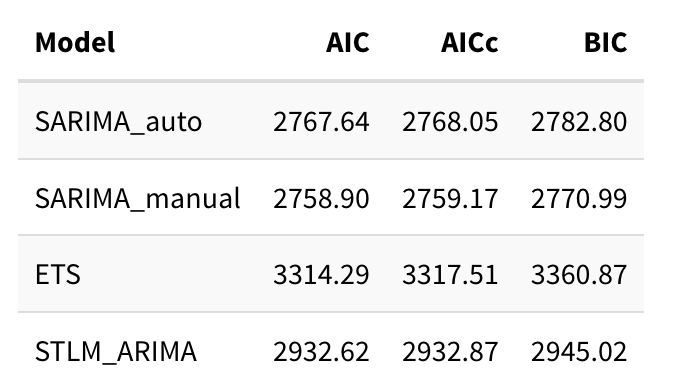
\includegraphics[width=0.75\linewidth]{images/table1.png}
    \caption{Comparison of Information Criteria across Models}
    \label{fig:enter-label}
\end{figure}

When the AIC, AICc and BIC criteria are compared between the models, it can be seen that the SARIMA\_manual model has the lowest values for all metrics, indicating a better balance between fit and model complexity. The SARIMA\_auto model performed similarly, but slightly less well. In contrast, the STLM\_ARIMA and ETS models had significantly higher values, suggesting that they fit the data less efficiently, possibly due to greater complexity or an inability to capture the patterns in the series. Therefore, based on the information criteria, the SARIMA\_manual model is the most suitable for this time series.

\subsection{Model Comparison Based on Forecast Accuracy}
To evaluate the predictive ability of the various models, we examined the error metrics in the test set. The metrics considered were RMSE (root mean squared error), MAE (mean absolute error), MAPE (mean absolute percentage error) and Theil's U. These metrics provide different perspectives on the quality of the forecasts.

The table below summarises these metrics for the four evaluated models: SARIMA with automatic parameter selection (SARIMA\_auto); SARIMA with manual parameters (SARIMA\_manual); the ETS model; and the hybrid STLM model with ARIMA in the residuals (STLM\_ARIMA). The aim of this comparison is to identify the model with the best predictive performance and the lowest error in forecasting future values of the series.

\begin{figure}[H]
    \centering
    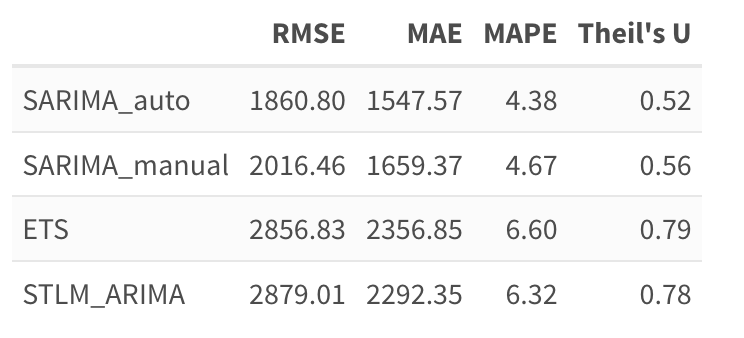
\includegraphics[width=0.75\linewidth]{images/table2.png}
    \caption{Forecast Accuracy Comparison on Test Set}
    \label{fig:enter-label}
\end{figure}

When the models were compared based on the forecasting metrics in the test set, the SARIMA\_auto model exhibited the best overall performance, showing the lowest RMSE, MAE, MAPE and Theil's U values. This indicates greater accuracy and better predictive capacity. SARIMA\_manual performed reasonably well, albeit slightly less well than the automatic model. The ETS and STLM\_ARIMA models, on the other hand, produced significantly higher error values, suggesting that they are less effective for forecasting this series. Therefore, the automatic SARIMA model is the most suitable choice for future forecasting.

\subsubsection{Forecast Visualisation}
In addition to quantitative metrics, visually comparing the predictions with the actual data is fundamental to understanding how each model behaves over time. The graph below shows the actual values of the test set alongside the forecasts generated by each model.

This visualisation enables us to identify any systematic deviations, as well as the models' ability to capture seasonality and trends, and any delays or one-off errors in the forecasts.

By comparing the model forecasts with the actual data, we conclude that SARIMA\_auto and SARIMA\_manual produced the most accurate predictions.

\begin{figure}[H]
    \centering
    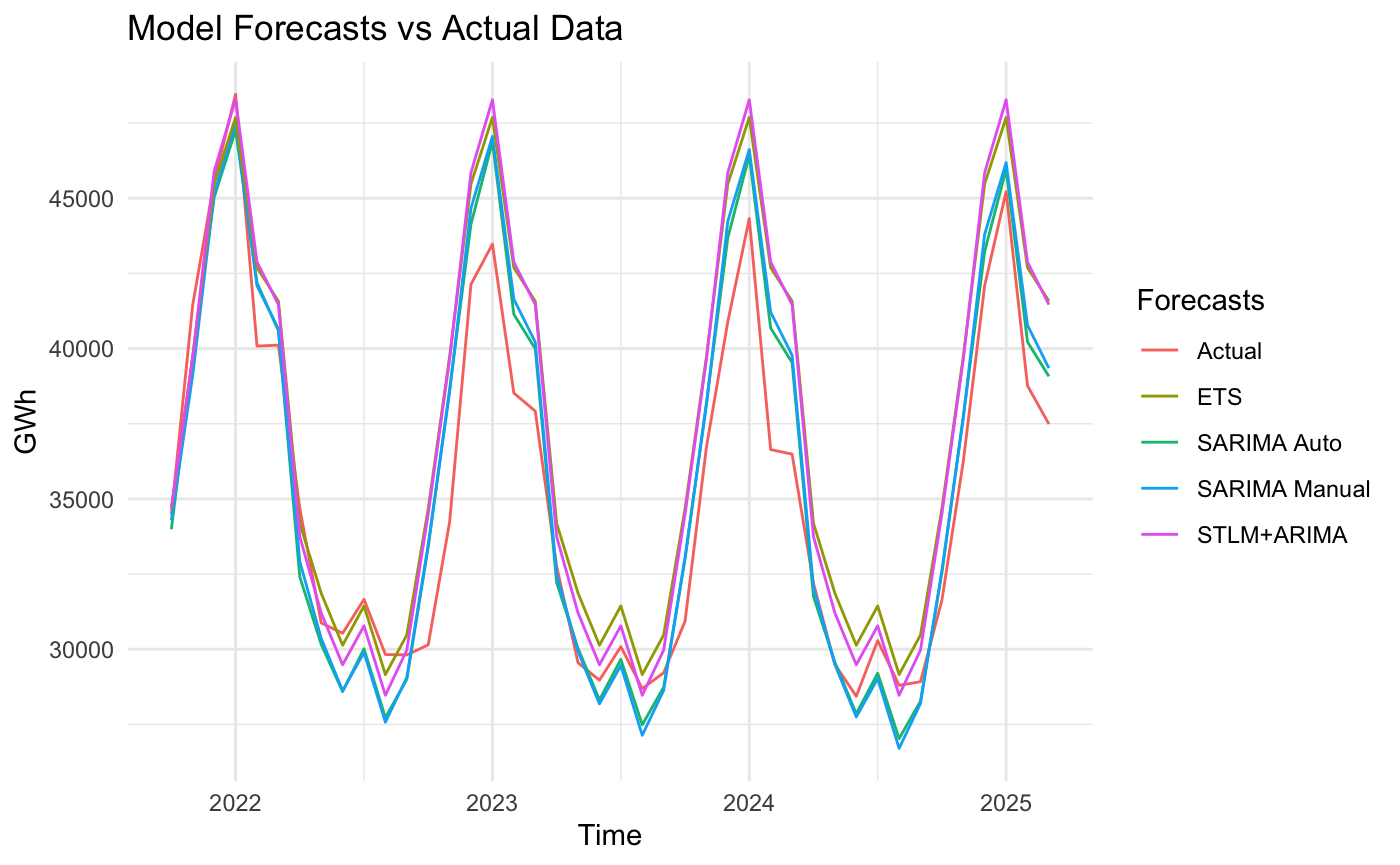
\includegraphics[width=1\linewidth]{images/grafico_fixe.png}
    \caption{Forecast Visualisation of the four models}
    \label{fig:enter-label}
\end{figure}

\section{Conclusion}
When analysing the information criteria (AIC, AICc and BIC) and forecast accuracy metrics (RMSE, MAE, MAPE and Theil's U) in the test set, the SARIMA\_auto and SARIMA\_manual models emerged as the most suitable for modelling the time series.

SARIMA\_manual produced the lowest information criterion values, indicating the best balance between model fit and complexity. However, SARIMA\_auto obtained the lowest forecast errors in terms of predictive performance, suggesting greater capacity for generalisation and accuracy in future data.

Conversely, the ETS and STLM\_ARIMA models exhibited significantly higher values in both the information criteria and the error metrics, suggesting poorer model fit and forecasting performance.

Therefore, the ideal choice depends on the objective: SARIMA\_manual is more suitable for better historical adjustment, while SARIMA\_auto is superior for future forecasting with lower error. Overall, SARIMA models are more appropriate for this data than ETS and STLM\_ARIMA models. By comparing the models' forecasts with the actual data, we can conclude that SARIMA\_auto and SARIMA\_manual produced the most accurate predictions.